\chapter{Introduction}\label{chap:introduction}

The purpose of the project was to take a set of data collated by
members of the Life and Health Sciences department and to categorise
and store it online in an accessible form for other people to
search. There are many existing databases categorising biological
information at the molecular level, but none for the isoelectric point
(pI). The isoelectric point is the acidity (pH) at which a molecule
carries no net charge. Below the isoelectric point, proteins have a
net positive charge, above it a negative charge. In the denatured
state, the pI depends solely on a protein’s amino acid composition.

Professor Ian Nabney proposed the project and supervised
development. Dr Darren Flower of the Life and Health Sciences
department acted as the principle owner of PIP-DB, providing a copy
for use in the website. Additionally, he was responsible for helping
to explain the required biochemistry theory, and acted as a potential
user during design feedback sessions. The two primary deliverables
provided by Professor Nabney in the project description were:

\begin{enumerate}
\item An updatable relational database warehousing the provided dataset.
\item A web-accessible GUI with searching and downloading functionality.
\end{enumerate}

This meant that the aim of development would be to get a website
hosted online on a public server, accessible via a suitable web domain
address. The website should offer a service whereby users can search
PIP-DB and download search results using a web browser. This simple
and open-ended specification allowed for the majority of development
effort to be focused upon innovating on the areas of database driven
website development, and search engine usability.

The primary reason for choosing the project was that there is a real
existing need for a product of this type within the molecular biology
community, with potential value and use for future scientific
research. Development of database driven websites was an area which I
was unfamiliar with and had no prior experience in, but is a skill
that I felt was important to master.

This is an interdisciplinary project that involves aspects of web
application development, bioinformatics, data analysis, interaction
design, and data mining. The project plan used the OpenUP development
process, which places an emphasis on the early mitigation of
risks. Two sets of milestones were defined to govern project
development, covering the requirements of the design and
implementation aspects of the project. The design milestones were
given the labels D1 through D4 and the implementation milestones M1
through M3. Figure~\ref{fig:timeline} shows the chronology of
development.

\newpage
\begin{multicols}{2}

\section*{Objectives}\label{sec:objectives}
The following objectives were written during before the planning stage
of the project in order to provide a very high level overview of the
finished product, and to express personal goals and expectations for
the project which can then be refined to produce specific and
quantifiable requirements.

\begin{enumerate}
\item To build a free (as in freedom) web application for searching
  and viewing protein isoelectric points.
\item To produce a bioinformatics tool with real world value for
  future scientific research.
\item The application should provide intuitive but powerful searching
  facilities.
\item The application should provide a convenient means for a
  certified user to edit and upload additional data.
\item The application should present information in a usable and
  efficient form.
\item Users should be allowed to download generated results for
  offline use.
\item Adequate security precautions should be taken to minimise the
  risk of data being sabotaged or stolen.
\item The implementation should use a clean model view controller
  architecture.
\item Comprehensive test coverage of the API and common use cases
  should be automated.
\item The application should be scalable for much larger datasets.
\end{enumerate}

\noindent
Chapter~\ref{chap:requirements} includes a description of the
requirements derived from these objectives, and
Chapter~\ref{chap:evaluation} evaluates the project with reference to
the objectives, offering a measure of achievement for each. See the
Overview section for a thorough description of the document structure.

\columnbreak

%%%%%%%%%%%%%%%%%%%%%%
%% Figure: timeline %%
%%%%%%%%%%%%%%%%%%%%%%
\begin{figure}[H]
\centering
% The bizarrely-specific height value is to vertically align the
% caption with the left column text:
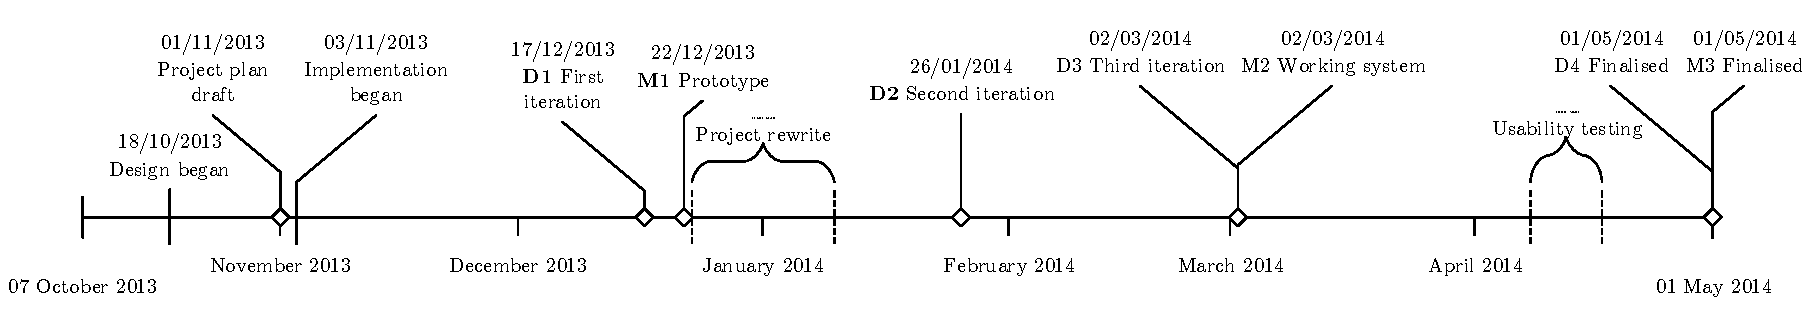
\includegraphics[angle=90,origin=c,height=0.4561\paperheight]{assets/timeline}
\caption[Project development timeline]
        {A timeline of project development, showing significant major
          project milestones.}
\label{fig:timeline}
\end{figure}

\end{multicols}

\newpage

\newpage
\section*{Submission archive}
The accompanying archive for this report contains a snapshot of the
development repository. It was prepared automatically using the
\texttt{mksubmission.sh} script written for this purpose. While every
effort has been made to include relevant source code listings in this
report, it is intended that a curious reader will investigate the
contents of the archive of their own accord, as the large size of the
source code means that only a small proportion can be reproduced in
this report. Figure~\ref{fig:dir-tree} identifies the key directories
that may be of interest to the reader. The diagram shows a directory
tree, where each directory has been annotated with numbers
corresponding to the sections which discuss them within this
report. The UNIX path delimiter ``/'' is used throughout this text,
with absolute paths referring to the root directory of the archive.

This is a polylingual project including source code written in Clojure
LISP, JavaScript, Less CSS, M4sh, Make, Python, and sh programming
languages. The documentation is formatted in \LaTeX, HTML and
Markdown. A reasonably competent text editor is all that is required
to view the source files, which can be identified by the file
extensions: ac, am, bib, clj, fsa, in, js, json, less, md, py, sh,
tex, xml, yml.

Note that while the submitted archive contains all project source
codes, the third party BLAST+ binaries and compilers JAR have been
removed in order to keep the size of the submission archive down.


%%%%%%%%%%%%%%%%%%%%%%
%% Figure: dir-tree %%
%%%%%%%%%%%%%%%%%%%%%%
\begin{figure}[H]
\begin{multicols}{2}
\centering
\hspace{1.5cm}\textbf{Archive directory}

\raggedleft
% LEFT COLUMN: Directory tree
\begin{tikzpicture}[dirtree]
\node {\texttt{/}}
child {node {\texttt{bin}}}
child {node {\texttt{build}}}
child {node {\texttt{Documentation}}
  child {node {\texttt{design}}}
  child {node {\texttt{evaluation}}}
  child {node {\texttt{midterm}}}
  child {node {\texttt{plan}}}
  child {node {\texttt{report}}}
}
child {node {\texttt{extern}}}
child {node {\texttt{resources}}
  child {node {\texttt{css}}}
  child {node {\texttt{fonts}}}
  child {node {\texttt{img}}}
  child {node {\texttt{js}}}
}
child {node {\texttt{scripts}}}
child {node {\texttt{src}}}
child {node {\texttt{test}}}
child {node {\texttt{tools}}
  child {node {\texttt{csv2yaps}}}
  child {node {\texttt{png}}}
  child {node {\texttt{watchr}}}
  child {node {\texttt{yaps2fsa}}}
};
\end{tikzpicture}
\columnbreak

\raggedright
\textbf{Sections in this document}

\textit{%
% RIGHT COLUMN: Section cross-references
\br{}\\ % /
\ref{sec:build-automation}\\ % /bin
\ref{sec:build-automation}\\ % /build
\ref{sec:development-process}, \ref{sec:design-process}\\ % /Documentation
\ref{sec:design-process}\\ % /Documentation/design
\ref{sec:usability-testing}\\ % /Documentation/evaluation
\ref{sec:development-process}, \ref{sec:programming-language-choice}\\ % /Documentation/midterm
\ref{sec:prototype-implementation}\\ % /Documentation/plan
\br{}\\                                    % /Documentation/report
\ref{sec:search-engine}\\ % /extern
\ref{sec:build-automation}\\ % /resources
\ref{sec:build-automation}\\ % /resources/css
\br{}\\                                    % /resources/fonts
\br{}\\                                    % /resources/img
\ref{sec:search-engine}\\ % /resources/js
\ref{sec:task-automation}\\ % /scripts
\ref{sec:prototype-rewrite}, \ref{sec:persistent-storage}, \ref{sec:search-engine}\\ % /src
\ref{sec:test-automation}\\ % /test
\ref{sec:task-automation}\\ % /tools/
\ref{sec:persistent-storage}\\ % /tools/csv2yaps
\ref{sec:test-automation}\\ % /tools/png
\ref{sec:build-automation}\\ % /tools/watchr
\ref{sec:persistent-storage}\\ % /tools/yaps2fsa
}
\end{multicols}
\caption[Archive directory structure]
        {Archive directory structure and report section cross-references.}
\label{fig:dir-tree}
\end{figure}

\newpage
\subsubsection*{Building the project}
A complete copy of the project can be compiled on a GNU/Linux
operating system by executing the command \texttt{./bin/build -{}-all}
from within the project root directory. This will invoke a script that
will attempt to automatically resolve system dependencies and
requirements. Failure to meet the system requirements will results in
an informative error message being displayed. See
Section~\ref{sec:build-automation} for further information.

\section*{Nomenclature}\label{sec:nomenclature}
Acronyms and initialisms will be used where appropriate in place of
full terms. When one is to be used, the first use of the term will
include the full expanded name, followed by the acronym in
parenthesis. The acronym will then be used from thereon in.


\subsubsection*{On the project name}
Throughout this text it is necessary to carefully distinguish
conversation about the biological dataset from the software and
algorithms used to host it. To achieve this distinction, I will use
the initialism PIP-DB to refer to the biological dataset assembled by
members of the Life \& Health Sciences department, and the
\textit{name} pip-db to refer to the software project that I developed
to host this. In order to keep this distinction clear, the
capitalisation will be kept consistent irrespective of the grammatical
context.


\subsubsection*{On the use of UML}
A subset of the Unified Modelling Language \cite{ibm2003uml} is used a
basis for many of the technical diagrams. One notable deviation from
convention is the use of sequence diagrams to describe the behaviour
of web services \cite{ibm2004sequence}. In such cases, the desired
effect is to illustrate the behaviour of a system at a high level, not
to provide a technically accurate description of communication.


\section*{Overview}\label{sec:overview}
The rest of the text is structured as follows: the project risk
assessment is described in Chapter~\ref{chap:risks}, with a brief
overview of the risks identified during the project planning phase and
a description of the mitigation strategies. A large body of text is
then devoted to a description of the design and implementation of the
final product, and is divided accordingly: information relevant to the
development process and work flow is described in
Chapter~\ref{chap:process}; the development of infrastructure and
tooling is described in Chapter~\ref{chap:infrastructure}; and the
product implementation in
Chapter~\ref{chap:product}. Chapter~\ref{chap:evaluation} contains an
evaluation of the software and the results of usability testing, and
the conclusions and recommendations for further work can be found in
Chapter~\ref{chap:conclusions}. The appendices begin at
page~\pageref{appendices}, followed by the bibliography and references
at page~\pageref{bibliography}. The purpose of the Requirements and
Process chapters is to offer an insight into the development plan and
workflow. A reader who is solely interested in the implementation and
engineering of the project may skip ahead to
Chapter~\ref{chap:infrastructure}.
